\chapter[High-Throughput Calculation]{High-Throughput Calculation} \label{c:tc3} 

\section{Introduction}

Hybrid organic-inorganic perovskites have attracted considerable attention in recent years due to their exceptional properties and ease in materials design, driving impressive advancements in photovoltaic and optoelectronic technologies [1-8]. Notably, the power conversion efficiency of three-dimensional (3D) perovskite solar cells has surged to 26.1\% [9], comparable to that of monocrystalline silicon solar cells [10]. However, the intrinsic instability under environmental stressors of these 3D perovskites has been the main obstacle that hinders their commercialization [11]. Driven by this, two-dimensional (2D) perovskites with fundamentally improved stability by incorporating large hydrophobic organic cations have been extensively studied [12-15]. Depending on the type of organic spacers employed, 2D perovskites are classified into Ruddlesden-Popper (RP) [13, 16], Dion-Jacobson (DJ) [17, 18] and alternating cation (ACI) phase perovskites [19, 20].  Among those phases, DJ perovskites, featuring one layer of divalent organic spacers between inorganic layers, have shown outstanding charge transport properties benefiting from the elimination of van der Waals gap [17, 18]. These 2D perovskites exhibit promising performance in optoelectronic applications including photovoltaics and light-emitting diodes [21]. A few groups reported efficiencies of 2D perovskite solar cells close to or even exceeding 20\% [22-24], and 2D perovskite light-emitting diodes have demonstrated high external quantum efficiencies of over 20\% [25, 26].

Unveiling the full potential of 2D perovskite-based devices hinges on a comprehensive understanding of their fundamental electronic properties. The unique layered structure of 2D perovskite with distinct inorganic and organic components naturally forms quantum wells where energy states are spatially localised [27]. Based on the energy level alignment between the two components, quantum wells are classified into four types: type $I_a$ and type $I_b$ (straddled gaps) where electrons and holes find their lowest energy within the same component; type $II_a$ and type $II_b$ (staggered gaps) where their lowest energies are in different components [28]. In the common wisdom, 2D perovskites typically exhibit a type $I_a$ quantum well, with the inorganic part as the potential well and the organic part as the potential barrier [29]. In principle, the organic and inorganic potentials can be tuned independently by composition control of organic and inorganic components. Yet, achieving different quantum well types in 2D perovskites is challenging due to the insulating nature of organic spacers with respect to the semiconducting nature of the inorganic framework [29]. Effective strategies have been demonstrated by using organic spacers with conjugated backbones featuring intrinsic semiconducting characteristics. In a series of representative studies, thiophene-based organic spacers with varying conjugation lengths have been incorporated into RP phase perovskites, achieving all four types of quantum wells [30-32]. Meanwhile, theoretical works also predicted the control of quantum well type in DJ phase perovskites by changing the conjugation length of thiophene-based [28] and benzene-based [33] organic spacers. Despite these efforts, the current explorations of conjugated organic spacers are still limited to a specific set containing a particular aromatic moiety. The constrained availability of experimentally obtained 2D perovskites restricts the exploration of organic spacers. There remains an open question regarding the selection of organic spacers from the extensive chemical space to achieve a specific quantum well type. 

In this work, by using high-throughput density functional theory (DFT) calculation, we unravel the intricate relationship between organic spacers and quantum well types in DJ perovskites. Leveraging the vast chemical space of organic spacers, we develop an open-source DJ perovskite repository containing 138 hypothetical compounds based on 11 existing structures. Using hybrid DFT calculations, we determine the electronic structure and extract the energy level alignment. Our findings demonstrate that type $I_a$ quantum well nature of 2D perovskites can be altered through the design of conjugated organic spacers, allowing for the achievement of all four types of quantum wells by fine-tuning the organic potentials. To guide the systematic design of organic spacers, we propose two design principles: electron richness and degree of $\pi$-conjugation, as key considerations for selecting organic functional groups. We hope that the insights gained from this work could guide and stimulate further exploration of diverse organic spacers in 2D perovskite research. 

\section{High-throughput Workflow}

The conventional approach to materials discovery and advancing our understanding of functional materials involves the laboratory synthesis of new compounds. Accelerating progress in the field of 2D perovskites would greatly benefit from access to a diverse array of potential 2D perovskite materials. While substantial knowledge has been accumulated in recent years concerning 2D perovskites [34, 35], databases exclusively dedicated to experimentally obtained phase-pure N=1 DJ-type 2D perovskites remain limited and sparse. While hypothetical structures have been proposed through DFT calculations [28, 33], the majority of these studies have focused on a restricted set of organic spacers, often derived from a single experimentally available prototypical spacer. This approach leaves a significant portion of chemical space unexplored. High-throughput computational methods represent a powerful tool for navigating the materials space and for screening materials without the expense of trial-and-error materials synthesis in the laboratory [36-39]. This approach has demonstrated considerable success in the screening of stable RP-type 2D perovskites [40] and in the evaluation of promising perovskite-derived materials for optoelectronics [41]. 

To overcome the challenges posed by data scarcity and the limited number of experimentally obtained structures for DJ perovskites, we adopt a high-throughput DFT calculation workflow, as illustrated in Fig. \ref{f:fig1}. This workflow sets itself apart from prior methodologies by taking into consideration all conceivable combinations of fundamental building blocks of organic functional groups, resulting in an extensive array of organic spacer candidates. Considering the vast chemical space associated with divalent organic spacers, we recognize that performing hybrid DFT calculations on each candidate is impractical. Therefore, we employed a strategy to refine our focus by identifying representative structures that are essential for comprehending their behaviour. In our study, two crucial functional groups are identified as essential building blocks for organic spacers: $\pi$-conjugated backbones and non-conjugated alkyl group [35]. Firstly, $\pi$-conjugation is the key to open possibilities for different types of quantum wells in 2D perovskites [30]. Previous studies have demonstrated that non-conjugated spacers, such as alkyl organic spacers, exhibit frontier levels hidden far behind the inorganic band edge, leading to type $I_a$ alignment [35]. To bring forward the organic frontier levels, we introduce $\pi$-conjugation into the organic spacer by using ring-shaped backbones, which may comprise monocyclic or fused/linked polycyclic rings [28, 30]. Secondly, the presence of anchoring alkyl group is essential for ensuring the structural stability of 2D perovskites [35]. The 2D layered structure is stabilized through the formation of ionic bonds between the positively charged organic spacer and negatively charged inorganic layer. The positive charges on the organic spacer can take the form of an anchoring alkylammonium group attached to the backbone or a protonated nitrogen substituting the carbon on the backbone [18, 42]. In the case of DJ perovskites, which require two positive charges, it has been observed that at least one alkylammonium is crucial for the formation of the 2D layered structure [43]. Building upon these two prerequisites, aromatic units and alkyl groups can be combined, with certain constraints dictated by the formability of 2D perovskites, including spacer size and shape. For example, the size of backbones must be smaller than the inorganic octahedra to fit into the 2D perovskite structure [44]; and the position of protonated nitrogen should accommodate the cavity within neighbouring inorganic layers [45]. Derived from these considerations, we generate 138 hypothetical compounds, each featuring organic spacers sandwiched by one layer of $PbI_6$ as the inorganic framework, to comprehensively explore the behaviour of organic spacers in the electronic structure of 2D perovskites. 

\begin{figure}[!ht]
\centering
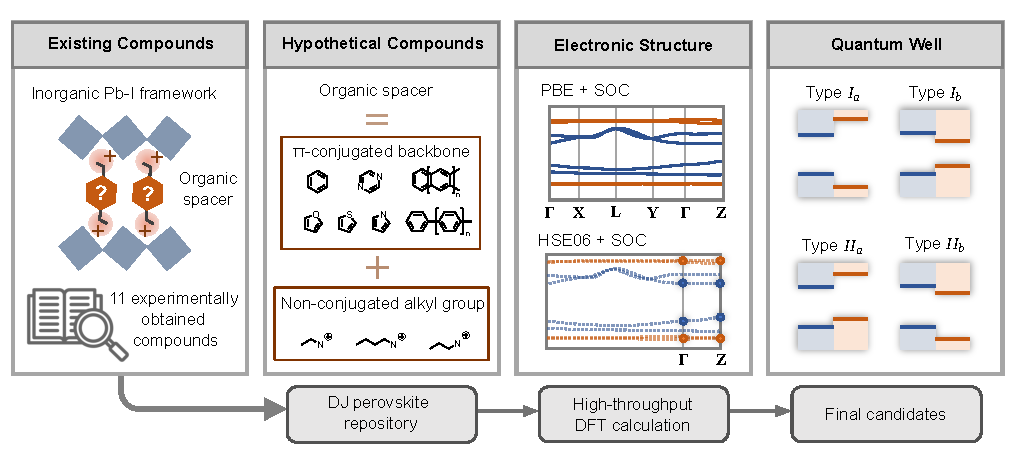
\includegraphics[width=\textwidth]{figures/high-throughput-calculation/figure1.pdf}
\caption[Schematic diagram of the high-throughput calculation workflow.]{Schematic diagram of the high-throughput calculation workflow. Our study focuses on DJ perovskites with a model structure comprising divalent organic spacers sandwiched between single layers of inorganic PbI6 octahedra. Based on 11 existing compounds, we generate a DJ perovskites repository containing 138 hypothetical compounds. We consider two essential building blocks for organic spacers: $pi$-conjugated backbone and non-conjugated alkyl group. Electronic structures calculations employ PBE+SOC to validate band shape, while HSE06+SOC are used at specific points to match bandgap value accurately. Energy level alignments are derived and final candidates with all four types of quantum wells are identified. }
\label{f:fig1}
\end{figure}
 
The computational challenge associated with DFT calculations of 2D perovskites stems from the complexity of their crystal structure, which typically involves more than 100 atoms within a unit cell. As a result, our objective is to strike a balance between computational cost and accuracy in our simulation. To achieve this objective, we rely on making juristic choices on two aspects: an appropriate unit cell and the level of theory employed.

(1) Unit cell selection: To simplify the complex 2D perovskite structure while preserving symmetry, we aim to employ the smallest simulation cell that captures the average disorder in both organic and inorganic components. To achieve this, we reference the previously reported experimental structure measured by X-ray diffraction. In the case of 2D perovskites, the experimentally determined unit cell typically consists of up to four octahedral units due to the lower symmetry introduced by the organic spacers, in contrast to the two-octahedra units observed for 3D perovskites [18, 42]. In this study, we select a unit cell that comprises four octahedra units arranged in a 2x2x1 configuration, a choice commonly employed in previous DFT simulations [33, 46]. In terms of the packing of organic spacers, it has been observed that smaller spacers tend to align out-of-phase (with neighbouring spacers along the a- and b-axes in-plane directions, respectively) [18, 42], while larger spacers may also align in-phase (with neighbouring spacers along a-axes in-plane direction) [30]. To ensure consistency across our repository, we opt for the former configuration, as previous simulations have demonstrated that it minimises the dipole moment and results in the lowest formation energy [47, 48].  

(2) Level of theory: A generally accepted simulation protocol derived from previous DFT calculations on 2D perovskites is to choose the GGA (PBE) functional for structural calculations, and the more accurate yet computationally expensive hybrid (HSE06) functional to accurately capture the experimental bandgap value [28, 33]. Additionally, it is well established that the inclusion of spin-orbit coupling (SOC) is necessary to accurately describe the band dispersion of the heavy Pb atom [33, 49]. In this work, performing hybrid functional calculations for the electronic structure of 2D perovskites across the entire Brillion zone is computationally challenging. We overcome this computational bottleneck by using a combined approach of PBE and HSE06 functional for electronic structure calculation. We observe that upgrading the theory from GGA+SOC to HSE06+SOC only shifts the energy level of each band without altering the band shape. To reduce computational costs, we perform electronic structure calculations using PBE +SOC across the Brillion zone to identify the dispersion of the bands. On top of that, HSE06+SOC hybrid functional calculations are conducted on $\Gamma$ and Z points in reciprocal space to match the experimental band gap [18, 42, 50-55]. A mixing factor of 0.40 is chosen for hybrid functional resulting in an average deviation of approximately 0.05 eV from experimentally obtained values (Table S2). Further computational details on crystal structure and level of theory can be found in SI Section II. 

\section{DJ Perovskite Repository}

Our open-source DJ perovskite repository is shown in Fig. \ref{f:fig2}, expanding the landscape of spacers from 11 existing compounds [18, 42, 48, 50, 51, 53-55] to 138 hypothetical compounds (see the full list of spacers in SI Section I). The repository is publicly accessible through the Materials Project Website. We recognize that the variations in chemical structures of organic spacers posit a much larger ensemble than the repository, encompassing factors such as the types and numbers of aromatic units [30, 54], length and position of alkyl groups [18, 45], heteroatom substitution [55], and the repeating patterns of the aromatic units [33], among others. Indeed, the permutations and combinations of these structural motifs offer a diverse array of organic spacers. Unlike the previously reported repository for other materials that often involve hundreds or even thousands of structures [40], the high computational cost of hybrid DFT calculation of 2D perovskites limits our ability to simulate every possible structure within the chemical space. To confront this challenge, we adopt a hierarchical approach to navigate the extensive materials space. First, we classify the spacers into two main groups: monocyclic and polycyclic spacers, based on the count of aromatic units within the organic spacer. This classification effectively distinguishes conjugated organic spacers from one another in terms of geometry, and more importantly, the electronic structure which is the key focus of our study. Both main groups are built upon the foundation of four basic aromatic units (benzene, thiophene, furan, pyrrole) as the backbone, with methylammonium as the alkyl group. Next, we move down the hierarchy from the main groups to subgroups by introducing slight modifications to the organic spacers, a commonly employed approach to select organic spacers in previous studies. Specifically, the monocyclic spacers main group further branches into two subgroups, considering modifications in heteroatom substitution [54, 55], and change in position and length of alkyl group [45, 53], respectively. Similarly, the polycyclic spacers main group is further divided into two subgroups, stemming from mutations in the repeating pattern of aromatic units [30, 33] and the incorporation of mixed aromatic units within the conjugated backbone [54], respectively. This hierarchical framework enables us to efficiently explore the diversity of organic spacers and derive insights into their design principles. 

\clearpage
\begin{figure}[!ht]
\centering
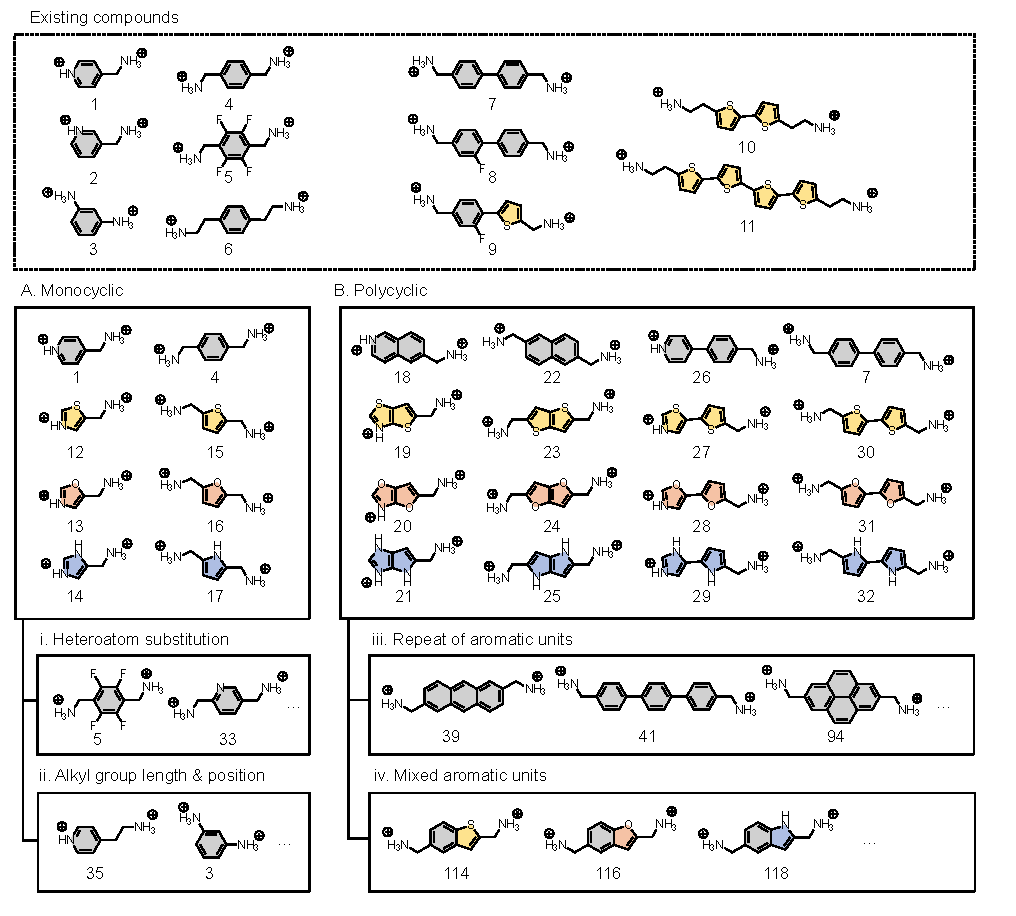
\includegraphics[width=\textwidth]{figures/high-throughput-calculation/figure2.pdf}
\caption[The DJ perovskites repository.]{The DJ perovskites repository. Starting with 11 existing compounds, we derive a total of 138 hypothetical compounds. The repository is structured hierarchically, consisting of two main groups, each further branching into two subgroups. We construct the repository based on four basic aromatic units: benzene (grey), thiophene (yellow), furan (orange), and pyrrole (blue), along with their derivatives. Main group A comprises monocyclic spacers using four basic aromatic units as the backbone and methylammonium as the alkyl group. Main group B includes polycyclic spacers with double aromatic units in linked and fused arrangements. Subgroup i encompasses monocyclic spacers with heteroatom substitution, including nitrogen substitution and fluorination. Subgroup ii involves monocyclic spacers with variations in alkyl group length and position. Subgroup iii incorporates polycyclic spacers containing more than two aromatic units and diverse fused patterns of aromatic units. Subgroup iv features polycyclic spacers with mixed types of aromatic units within the backbone. }
\label{f:fig2}
\end{figure}

\section{Modulation of inorganic and organic potentials} 

Fig. \ref{f:fig3}a illustrates the model crystal structure of DJ perovskites, along with its unit cell and corresponding first Brillouin zone in reciprocal space. Despite the intricate nature of 2D perovskite structures, their electronic band structures can be effectively captured by two crucial structural descriptors. One is the structural distortion of the inorganic framework, characterized by bond lengths and angles. Previous works have affirmed that Pb-I-Pb and I-Pb-I bond angles serve as the primary determinant of bandgap change, similar to 3D perovskites [46, 47, 56]. The other one is the interlayer separation of inorganic layers, which is dictated by the length of the organic spacer. This distance significantly influences the charge transport characteristics in the out-of-plane direction. Further analysis is conducted in the Brillouin zone, focusing on properties at the $\Gamma$ and Z points. 

\begin{figure}[!ht]
\centering
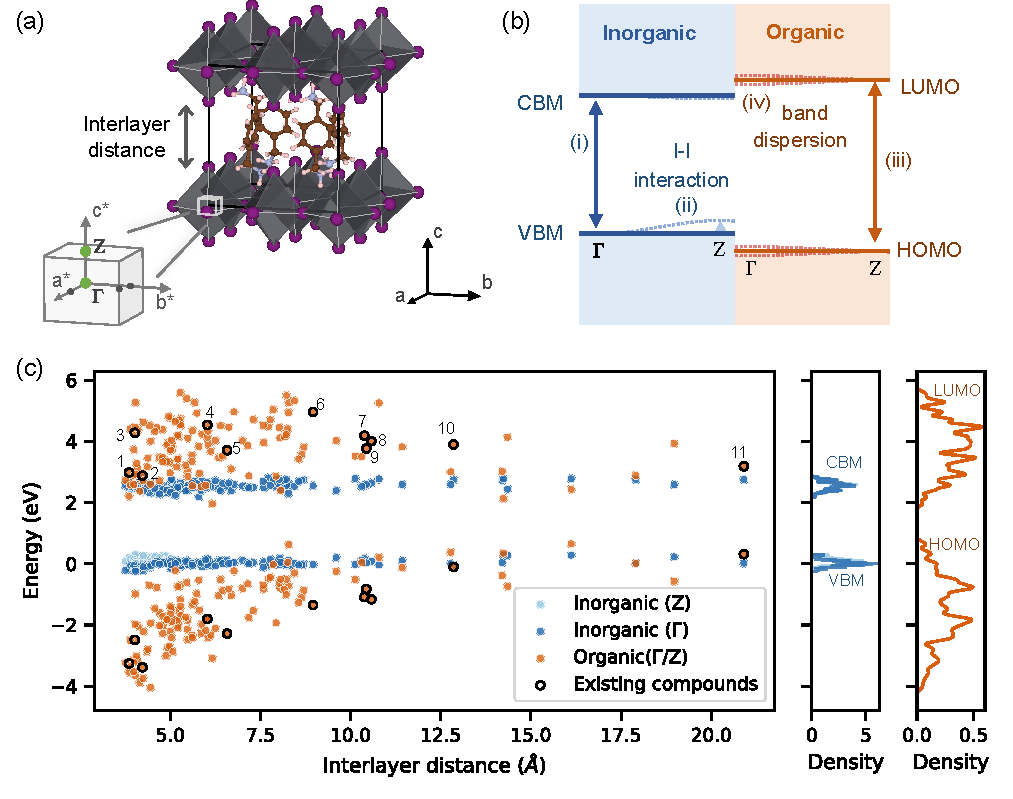
\includegraphics[width=\textwidth]{figures/high-throughput-calculation/figure3.pdf}
\caption[Modulation of inorganic and organic potentials in 2D perovskite quantum wells by organic spacers.]{Modulation of inorganic and organic potentials in 2D perovskite quantum wells by organic spacers. (a) 2D perovskite crystal structure and first Brillion zone. (b) Schematic quantum well diagram. The inorganic (blue) and organic (orange) potentials are modulated by four factors. $\Gamma$ and Z points indicate electron dispersion along the c direction. (c) Energy level alignments of all DJ perovskites calculated by HSE06+SOC plotted against interlayer distance. Comparison among the distribution of CBM, VBM, HOMO, and LUMO are plotted on the right. The energy levels of different perovskites are calibrated using Pb 1s orbital [67]. The average of the inorganic valence band maximum is taken as the zero of energy. CBM: conduction band minimum. VBM: valence band maximum. HOMO: highest occupied molecular orbital. LUMO: lowest unoccupied molecular orbital.}
\label{f:fig3}
\end{figure}

In 2D perovskites, quantum confinement arises from the alternation of organic and inorganic layers, leading to localized energy states in distinct layers. The energy state mismatch between the inorganic and organic layers gives rise to the quantum well configuration, as depicted in Fig. \ref{f:fig3}b. To define the edge states, we use conduction band minimum (CBM) and valence band maximum (VBM) for the continuous bands within the inorganic components. In contrast to the inorganic components, the organic components exhibit discrete energy levels with minimal dispersion. Therefore, we use the lowest unoccupied molecular orbital (LUMO) and highest occupied molecular orbital (HOMO) to define their frontier energy levels. Previous studies have indicated that the CBM and VBM are determined by the distortion of the inorganic framework, which varies based on the employed organic spacers [46, 47]. Manipulation of the organic frontier levels (HOMO and LUMO) can be tuned to potentially alter type $I_a$ quantum wells [28, 30]. However, the extent of these factors on the electronic structure and, by extension, the quantum wells remain unclear. Our simulations reveal that the modulation of the quantum wells by organic spacers can be distilled into four factors, accompanied by a quantitative comparative assessment.

The organic spacer indirectly influences the inorganic potentials (CBM and VBM) through two distinct factors:

(i) Within the in-plane direction, the bands exhibit dispersion along the a* and b* directions within the Brillion zone, converging at the $\Gamma$ point. This dispersive behaviour suggests facile carrier transport within individual inorganic layers, resembling the characteristics of 3D perovskites. In line with prior research, the VBM-CBM gap at $\Gamma$ point is contingent on the structural distortion of the inorganic framework [46, 47]. A larger disxtortion of the inorganic framework, characterized by smaller Pb-I-Pb and I-Pb-I bond angles, leads to a wider VBM-CBM gap. Our structural relaxation results indicate that these bond angles typically fall within the range of 140$^{\circ}$ to 170$^{\circ}$ for Pb-I-Pb and 160$^{\circ}$ to 180$^{\circ}$ for I-Pb-I bond angles, aligning with previous experimental and simulated values [18, 42, 46, 47, 56]. Within this distortion range, the variation of the VBM-CBM gap spans approximately 0.9 eV (Fig. S8).

(ii) In the out-of-plane direction, most compounds exhibit no dispersion from the $\Gamma$ point to the Z point. This implies limited charge transport between adjacent inorganic layers. However, an exception arises when the interlayer distance is minimized due to short organic spacers. This short interlayer distance results in a small band dispersion that signifies the interaction of iodide atoms between adjacent layers, aligning with previous findings [22]. Furthermore, we quantitatively establish that this dispersion is evident when the interlayer distance falls below 5 {\AA}, and it increases linearly as the interlayer distance decreases. Our repository encompasses DJ perovskites with interlayer distances down to 4 {\AA}, yielding a band dispersion of 0.5 eV at this level (Fig. S9).

The organic spacer directly influences the organic potentials (HOMO and LUMO) through another two factors:
(iii) The position of HOMO and LUMO is directly affected by the chemical structure of the organic spacer (Fig. S10). Depending on the functional groups contained within the organic spacer, the extent of modulation in HOMO and LUMO can span a range of several eV. Further elaboration on the design principles of organic frontier levels is provided in the subsequent section. 
(iv) The organic frontier levels exhibit minimal dispersion across the Brillion zone. Notably, we have observed that a packing arrangement of organic spacers with lower symmetry, resulting in higher ground state energy, can lead to dispersion in specific molecular orbitals of up to 0.8 eV (Fig. S10). Previous studies also indicate that this dispersion is influenced by the packing structure of the organic spacers, with a preference for minimal dispersion energetically [48]. Throughout this study, we assume that the band dispersion is negligible across all organic molecular orbitals, resembling the behaviour of isolated cations with negligible $\pi$-$\pi$ interactions between neighbouring organic spacers. 

In Fig. \ref{f:fig3}c, we present an overview of the energy level alignment of all DJ perovskites, plotted against the interlayer distance. Our simulations validate the prevailing understanding that 2D perovskites primarily exhibit quantum well structure. The inorganic potential changes a scale of several tens of eV. These changes result from variation in the bandgap at $\Gamma$ point due to inorganic framework distortion, as well as the narrowing of the bandgap at Z point when interlayer distance is small. As for the organic frontier levels, their dispersion remains negligible, while their position experiences significant changes, spanning several eVs across different compounds. This quantitative assessment leads us to the conclusion that the most effective strategy for engineering the quantum wells of 2D perovskites is the modulation of the organic frontier levels.

\section{Design principles for organic frontier levels}

Given that the frontier level of organic spacers is the most important strategy to tailor the quantum wells, we next demonstrate how to tune the frontier levels of organic spacers. Although the frontier levels design of organic spacers for 2D perovskites has only been mentioned in limited literature [28, 30, 32, 44, 50], the design of molecular orbitals has been well-developed in the field of organic semiconductors using established organic chemistry principles [57, 58]. From our high-throughput DFT calculation, we identified two key organic chemistry principles, namely electron richness and degree of conjugation, to engineer the frontier levels of organic spacers. Fig \ref{f:fig4} illustrates several representative organic molecules to comprehend these two design principles.

\begin{figure}[!ht]
\centering
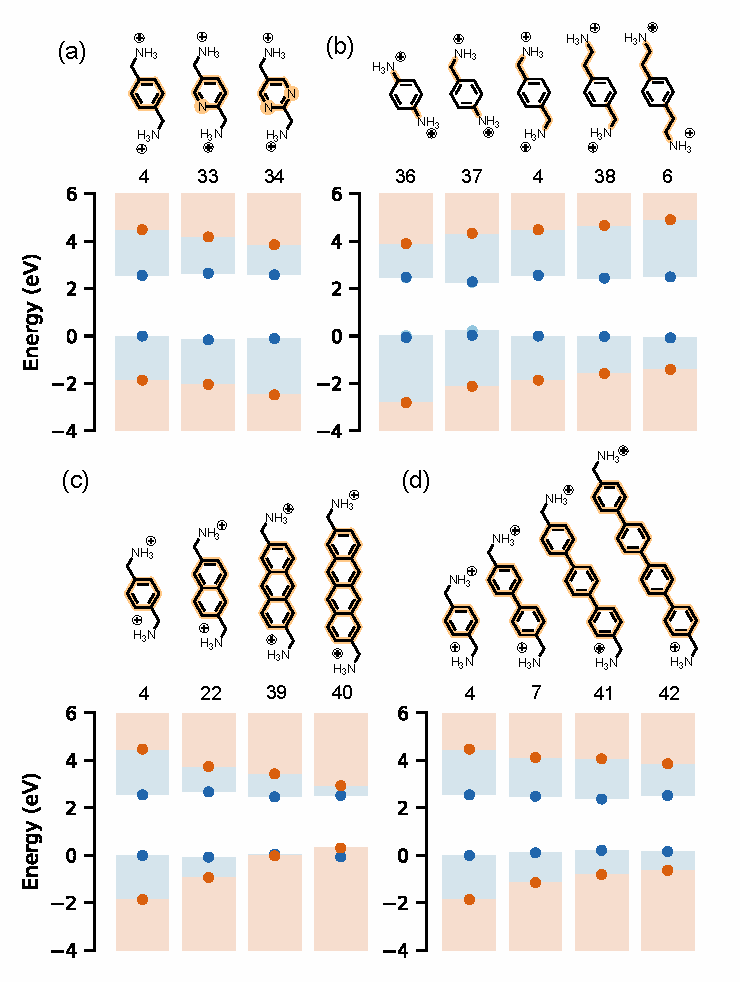
\includegraphics[width=0.6\textwidth]{figures/high-throughput-calculation/figure4.pdf}
\caption[Design principles for organic frontier level based on functional groups within organic spacers.]{Design principles for organic frontier level based on functional groups within organic spacers. Shifts in HOMO and LUMO positions due to variations in electron richness, demonstrated by (a) aromatic units and (b) alkyl group numbers and lengths. Reduction in HOMO-LUMO gap with increased $pi$-conjugation, exemplified by benzene-based spacers connected by (c) fusion or (d) linking. The functional groups of interest are highlighted on the chemical structure of the organic spacer. See Fig. \ref{f:fig3} b-c for colour coding of energy level alignment for further context.}
\label{f:fig4}
\end{figure}

Electron richness refers to the tendency of a molecule or atom to donate or withdraw electrons, and it plays a crucial role in determining the relative position of the frontier levels of the organic spacers [57]. By selecting electron-rich or electron-poor functional groups, we can achieve higher or lower frontier levels, respectively. This design rule is exemplified using monocyclic spacers, which consist of two building blocks: the aromatic unit (Fig. \ref{f:fig4}a) and the alkyl group (Fig. \ref{f:fig4}b). For instance, in six-membered rings, replacing carbon with more electronegative nitrogen in benzene rings (as seen in pyridine and pyrimidine) shifts the frontier levels downward [59]. Similarly, among common five-membered rings, replacing thiophene with electron-rich furan, or pyrrole raises the frontier levels (Fig. S12). Apart from the aromatic units, the alkyl group, exhibiting electron-rich behaviour, also offers a handle to shift the frontier levels. As an example, organic spacers with longer or multiple alkyl group exhibit higher frontier energy levels. 

The second design rule centres around the degree of $pi$-conjugation within the organic spacers. $pi$-conjugation is established through the overlapping of $pi$-orbitals in the backbone which aligns perpendicular to the ring [57, 58]. This overlap facilitates electron delocalization across adjacent aligned $pi$-orbitals, leading to a reduction in the HOMO-LUMO gap. Monocyclic spacers typically have a ubiquitous HOMO-LUMO gap of approximately 7~8 eV due to the comparable electron delocalization in the $pi$-conjugated aromatic unit. However, increasing the number of aromatic rings in the $pi$-conjugated backbone expands the region of overlapping $pi$-orbitals, enhancing electron delocalization and subsequently reducing the HOMO-LUMO gap [57]. The extent of this gap reduction depends on the spatial distribution of these $pi$-orbitals, which is governed by the geometry of the backbone. The geometry can be typically in the form of six-membered rings or five-membered rings connected through fusion or linking, as demonstrated in our investigation of benzene- and thiophene-based series (Fig. \ref{f:fig4}c). Among the studied series, the most effective narrowing of the HOMO-LUMO gap is achieved with ortho-fused benzene rings arranged in a rectilinear manner (refer to Fig. S5 for different spatial arrangements of fused benzene rings).

By employing these two design strategies, we can effectively tailor the frontier levels of organic spacers to manipulate the energy level alignment of 2D perovskites, enabling precise control over the behaviour of charge carriers. This approach offers promising opportunities for customizing the electronic properties of 2D perovskites for specific optoelectronic applications.

\section{Final candidates for all four types of quantum wells}

In this section we demonstrate the application of the design principles for organic frontier levels to modify the quantum well nature of 2D perovskites, showcasing the feasibility of achieving all four types of quantum wells. While multiple compounds exhibit each type of quantum well (Fig. S7), we highlight representative candidates with relatively short interlayer distances. Additionally, we present the artificial energy level alignment of quasi-2D perovskites containing up to four inorganic layers with experimentally measured energy level alignment [60], to offer a comprehensive insight into these quasi-2D perovskites.

\begin{figure}[!ht]
\centering
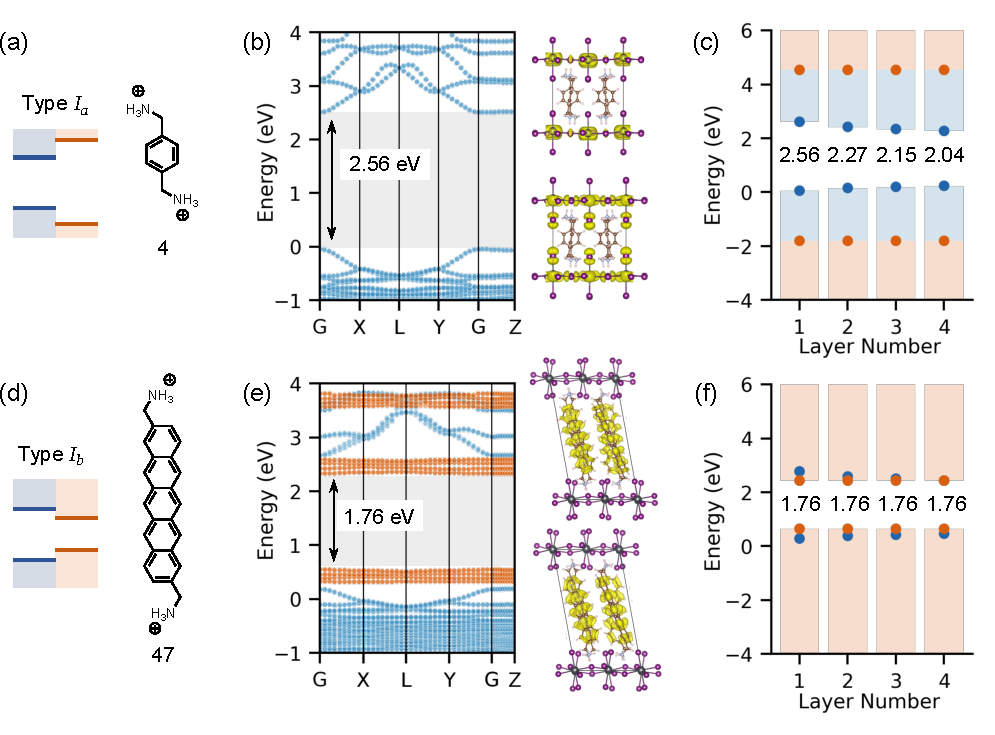
\includegraphics[width=\textwidth]{figures/high-throughput-calculation/figure5.pdf}
\caption[Final candidates for type I quantum well.]{Final candidates for type I quantum well. (a/d) Representative organic spacer with type $I_a$ / type $I_b$ quantum well. (b/e) The corresponding band structures are calculated using PBE+SOC bands scissored by HSE06+SOC energy levels. The charge density distribution of edge states is calculated using HSE06+SOC (showing 2 states per $APbI_4$ formula).  (c/f) Artificial energy level alignments for corresponding quasi-2D perovskites with inorganic layer number N=1~4 aligned using experimental values [60].  }
\label{f:fig5}
\end{figure}

Type $I_a$ quantum well features inorganic states at the band edge, typifying the most common energy level alignment in existing compounds. The majority of compounds in our DJ perovskite repository exhibit this quantum well type. Notably, although these perovskites demonstrate type $I_a$ quantum wells concerning the band edge at $\Gamma$ or Z point, certain compounds exhibit overlap between the organic and inorganic edge states due to the dispersive nature of the inorganic bands. This overlap leads to a transition from type $I_a$ towards type II quantum well. To ensure an explicit type $I_a$ configuration, the HOMO and LUMO must maintain a specific distance in energy from the inorganic band edge, with the LUMO positioned at least 0.4 eV above the CBM and the HOMO at least 0.3 eV below the VBM. Fig. \ref{f:fig5}a-c showcases a representative spacer with such characteristics, featuring Pb 6s orbital as the CBM, and Pb 6p and I 5s orbital as the VBM. The type $I_a$ quantum well persists with increasing inorganic layers, accompanied by a decrease in bandgap from 2.56 (N=1) to 2.04 eV (N=4).

Type $I_b$ quantum well exposes both organic frontier levels at the band edge, necessitating a small HOMO-LUMO gap. Achieve this involves increasing the conjugation length to bring the frontier levels into proximity. This can be realized through the elongation of any linked or fused spacer containing aromatic units. Among these possibilities, fused benzene rings represent the candidate with the shortest interlayer distance. As depicted in Fig. \ref{f:fig5}d-f, the band edge comprises the flat HOMO and LUMO bands, both originating from the overlapping $pi$-orbitals of the conjugated backbone. Upon incorporating more inorganic layers, the CBM and VBM gradually approach the organic frontier levels, resulting in a transition towards type $II_b$ quantum well while the bandgap remains consistent at 1.76 eV. 

\begin{figure}[!ht]
\centering
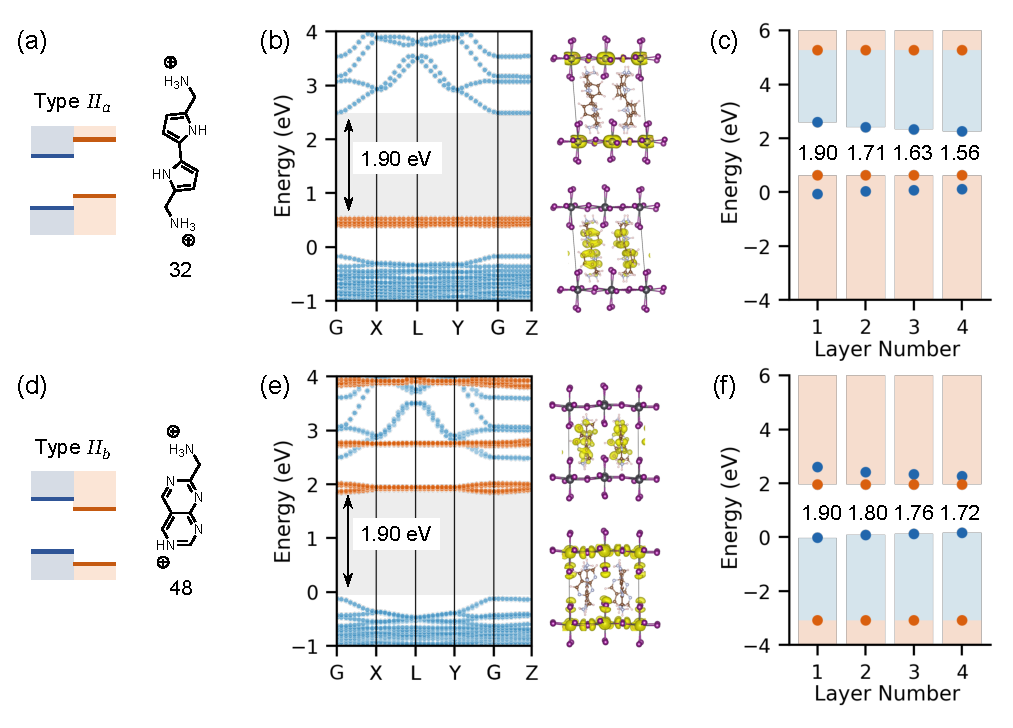
\includegraphics[width=\textwidth]{figures/high-throughput-calculation/figure6.pdf}
\caption[Final candidates for type II quantum well.]{Final candidates for type II quantum well. (a/d) Representative organic spacer with type $II_a$ / type $II_b$ quantum well. (b/e) The corresponding band structures are calculated using PBE+SOC bands scissored by HSE06+SOC energy levels. The charge density distribution of edge states is calculated using HSE06+SOC (showing 2 states per $APbI_4$ formula).  (c/f) Artificial energy level alignments for corresponding quasi-2D perovskites with inorganic layer number N=1~4 aligned using experimental values [60]. }
\label{f:fig6}
\end{figure}

Type $II_a$ quantum well exhibits a staggered gap with both organic frontier levels higher than the inorganic band edge. Achieving this requires an increase in conjugation length to reduce the HOMO-LUMO gap, combined with the use of electron-rich functional groups to lower the frontier levels. The selected candidate embodies a backbone of two linked pyrrole units and two alkyl group (Fig. \ref{f:fig6}a-c). This staggered configuration tailors the band gap to 1.90 eV. The band edge integrates a dispersive inorganic CBM constituted by Pb 6s orbitals, and a flat organic HOMO stemming from $pi$-orbitals in pyrrole units. The band shape implies decent electron mobility coupled with low hole mobility, contributing to the n-type nature of this compound. As the number of inorganic layers increases, the alignment remains intact, with the bandgap narrowing from 1.90 eV (N=1) to 1.56 eV (N=4).

Type $II_b$ quantum well also exhibits a staggered gap, with organic frontier levels lower in energy than the inorganic band edge. This alignment necessitates $pi$-conjugation in combination with electron-poor functional groups. Fig. \ref{f:fig6}d-f exemplify this using two fused benzene rings with nitrogen substitution as backbone, and one alkyl group. Similar to type $II_a$  alignment, the staggered confirmation also facilitates a reduction in the band gap to 1.90 eV. The band edge integrates a dispersive inorganic VBM constituted by Pb 6s orbitals, and a flat organic LUMO stemming from $pi$-orbitals in the conjugated backbone. Despite the minor band dispersion of LUMO, we assume this dispersion to be negligible in experimentally observed compounds (Fig. S11). The band shape implies low electron mobility and decent hole mobility, leading to the p-type nature of this compound. As the number of inorganic layers increases, the quantum well type remains consistent, accompanied by a reduction in the bandgap from 1.90 eV (N=1) to 1.72 eV (N=4).

\section{Organic spacer selection guidelines for PV application}

By leveraging the high-throughput DFT calculation of DJ perovskite, we have obtained a comprehensive understanding of how the organic spacer influences the energy level alignment of quantum wells. This understanding also comes with an in-depth understanding of bandgap and charge carrier behaviours in 2D perovskites. These insights are of great significance for practical applications, notably in the field of photovoltaics. In the vast landscape of literature surrounding 2D perovskite-based photovoltaics, the enhancement of PCE through compositional engineering has primarily centred on optimizing the charge transport properties along the out-of-plane direction. Within this context, two effective approaches have been identified. In the following discussion, we delve into these approaches, elucidating how our study contributes insights that validate these prior investigations and guide future research. 

The primary approach underscores the role of the inorganic component by minimizing the presence of organic components. This is achieved using short organic spacers, which effectively decrease the interlayer distance between adjacent inorganic layers. This strategy has been demonstrated widely in DJ and ACI phase perovskites [22, 24, 61, 62]. Remarkably, Aditya Mohite’s group adopted this strategy to achieve the highest PCE of 18.3\% among phase-pure 2D perovskite [22]. Their study highlighted that this approach is particularly effective in DJ and ACI phase perovskites, while the presence of the van der Waals gap in RP perovskites presents a challenge in achieving short interlayer distances. Our findings align well with this strategy, offering additional quantitative validation. Typically, this arrangement corresponds to type $I_a$ quantum well, attributed to the moderate HOMO-LUMO gap of short organic spacers. As the interlayer distance drops below 5 Å, an iodide-iodide interaction emerges between neighbouring inorganic layers, exhibiting a linear increase with decreasing interlayer distance. This interaction effectively reduces the bandgap and facilitates charge transport in the out-of-plane direction. Our repository includes organic spacers that result in interlayer distances down to 4.1 {\AA}. Notably, experimental reports indicate the potential for even shorter distances, reaching as low as 2 Å using alkyl linear and conjugated linear spacers [61, 63]. Our insights underscore the significance of adopting these short organic spacers to achieve effective out-of-plane charge transport and thus enhance device performance. Further exploration to ascertain the extent to which we can push interlayer distances while maintaining the stable 2D layered structure holds promise for future research. 

The second approach takes a distinct path by emphasizing organic components. It involves utilizing conjugated organic spacers to modify the insulating nature of the organic layer. For instance, Yongsheng Liu’s group explored the potential of conjugated organic spacers, such as thiophene-based monocyclic and polycyclic spacers, demonstrating that extended conjugation enhances the PCE of 2D perovskite-based solar cells up to 18.8\% [52, 64-66]. Their recent work attributes this conjugation to orbital interactions between organic and inorganic components [66]. Our investigation affirms that amplifying the degree of conjugation is the key to reducing the separation between organic frontier levels. Moreover, we establish two design principles to push these frontier levels beyond the band edge, resulting in an alternative quantum well configuration. Although this alternative type II quantum well theoretically offers benefits like efficient electron-hole separation and reduced bandgap [30, 32], charge carriers originating from the organic flat bands exhibit limited mobility, and the mechanism of light absorption in such compounds remains unclear. Nevertheless, considering the positive impact of conjugation on the PCE improvement [52, 65, 66], a deeper understanding of the effect of bringing organic frontier levels closer to or even beyond the band edge is warranted. Further exploration is required to elucidate how organic frontier levels impact light absorption and the subsequent charge transport processes, especially when these levels approach or exceed the band edge.

\section{Stability of the hypothetical compounds}

Validation of the synthesizability is crucial for guiding experimental research. Therefore, we calculated the formation energy of the four final candidates to confirm the stability of the hypothetical compounds. We assumed a synthetic route involving mixing iodized diammonium molecules $AI_2$ with $PbI_2$. Notably, all the formation energies of the hypothetical systems exhibit negative values of approximately -3.5 eV per APbI4 formula unit (Table S4). This aligns closely with the reported calculated formation energy of the experimentally available perovskites [33]. These results provide a primary indication that the experimental development of these 2D perovskites is feasible. 

Furthermore, the stability of our hypothetical perovskites is supported by recent literature, where high-throughput molecular dynamics simulations were used to examine the stability of thousands of hypothetical RP phase perovskites [40]. Their main focus was also on conjugated organic spacers with different numbers of repeated units. This investigation revealed high overall stability among these compounds, with most of the unstable perovskites featuring peripheral extra side-chain substitutions on the conjugated body of the polycyclic spacers. It is worth noting that we did not include such compounds in our repository. Additionally, we assume our DJ perovskites have higher overall stability, as it is well-known that DJ phase perovskites typically exhibit higher stability compared to RP types due to the absence of van der Waals gaps. While the aforementioned study suggests that the number of aromatic units is relatively unrestricted for successful perovskite incorporation, we are aware that as the number of aromatic units increases, the solubility of the organic precursor may become low due to strong $pi$-$pi$ interactions. This underscores the necessity for a careful design of the synthesis pathway for the hypothetical compounds in our repository.

\section{Conclusion}

In conclusion, our study employs high-throughput calculations on a collection of 138 DJ perovskites to unveil the pivotal role of organic spacers in tailoring the quantum well energy level alignment of 2D perovskites. Our simulations provide a quantitative assessment of the modulation of inorganic and organic potentials through incorporated organic spacers, revealing that the most effective strategy for engineering the energy level alignment of 2D perovskites is manipulating organic frontier levels. As effective means for tailoring these levels, we propose two design strategies, focusing on the electron richness of functional groups and varying degrees of $pi$-conjugation of the organic spacer. By implementing these design strategies, we successfully achieve all four types of quantum wells, unlocking the potential for charge carrier modulation. Furthermore, we shed light on how our study contributes insights into the selection of organic spacers, guiding future research on 2D perovskite-based photovoltaic. Ultimately, our work aims to inspire further experimental investigations into the integration of diverse organic spacers within the realm of 2D perovskite research.


